\subsection{Verso la Product Baseline}

\subsubsection{Pianificazione}
Periodo previsto: 16/01/2024-12/03/2024\\ 
\vspace{0.2cm} 
Periodo effettivo: (??)-(??)\\ 
\vspace{0.2cm} 
In questa sezione, pur avendo un'idea di ciò che ci attende, al momento abbiamo scelto di strutturare i nostri periodi di lavoro in fasi più lunghe anziché bisettimanali. Questa decisione deriva dalla nostra attuale valutazione delle competenze, poiché riteniamo prematuro definire l'intervallo che precede la seconda revisione con periodi di tempo molto definiti e stretti.

Le fasi attuali, più lunghe e meno specifiche, saranno progressivamente convertite in periodi bisettimanali quando vi sarà una maggiore consapevolezza delle \textit{attività}\textsubscript{\textit{G}} future.

\vspace{0.2cm}

\textbf{Obiettivo}: Nella fase successiva, il focus sarà sullo sviluppo dei Diagrammi delle Classi e sulla redazione di eventuali nuovi documenti. L'obiettivo primario sarà la realizzazione del prodotto effettivo partendo dal \textit{POC}\textsubscript{\textit{G}}, integrando le funzionalità non ancora implementate e migliorandolo nei punti più deboli della sua struttura.

\paragraph{Prima fase}
Intervallo temporale previsto: 16/01/2024-13/02/2024\\ 
\vspace{0.2cm} 
Durante la prima fase, l'attenzione sarà rivolta all'inizializzazione di possibili nuovi documenti per la \textit{PB}\textsubscript{\textit{G}}, in parallelo sarà affrontato lo studio dell'\textit{architettura}\textsubscript{\textit{G}} di \textit{sistema}\textsubscript{\textit{G}} e dei design \textit{pattern}\textsubscript{\textit{G}} più appropriati.

\vspace{0.2cm}

I lavori continueranno sul \textit{Piano di Progetto}, sulla correzione dei documenti \textit{Analisi dei Requisiti}, \textit{Glossario} e \textit{Piano di Qualifica}. Si avvierà la realizzazione dei diagrammi di \textit{attività}\textsubscript{\textit{G}} e sequenze, dando anche inizio allo sviluppo della prima versione del prodotto basata sul \textit{PoC}\textsubscript{\textit{G}}.

\paragraph{Seconda fase}
Intervallo temporale previsto: 13/02/2024-12/03/2024
\\ 
\vspace{0.2cm} 
Durante la seconda fase del progetto, l'attenzione sarà rivolta all’avanzamento di possibili nuovi documenti per la \textit{PB}\textsubscript{\textit{G}}, insieme alla continuazione dei documenti inizialmente avviati. In parallelo, saranno eseguite ottimizzazioni del \textit{sistema}\textsubscript{\textit{G}}, attraverso \textit{test}\textsubscript{\textit{G}} specifici per valutare la sua scalabilità e l'implementazione di allarmi per individuare eventuali anomalie o superamento di soglie critiche.

Si proseguirà con il perfezionamento del codice stesso, garantendo un costante miglioramento delle funzionalità e delle prestazioni del prodotto in fase di sviluppo.

\paragraph{Terza fase}
Intervallo temporale previsto: 12/03/2024-25/03/2024\\ 
\vspace{0.2cm} 
Durante la terza fase del nostro progetto, l'attenzione sarà rivolta all'ultimazione delle nuove versioni del \textit{Piano di Qualifica}, delle \textit{Norme di Progetto}, del \textit{Glossario} e del \textit{Piano di Qualifica}, completando contemporaneamente i documenti specifici della revisione \textit{PB}\textsubscript{\textit{G}}.

Sarà inoltre intensivamente testato il prodotto attraverso i \textit{test}\textsubscript{\textit{G}} e le metriche descritte all'interno del documento \textit{Piano di Qualifica} ed infine verrà creata la presentazione per la \textit{PB}\textsubscript{\textit{G}}.


%---------------------OTTAVO PERIODO---------------------------------------

\subsubsection{Ottavo periodo  16/02/2024 - 23/02/2024}
\paragraph{Considerazioni}

Gli obiettivi principali programmati per l’ottavo periodo riguardano l’esecuzione della seconda fase della revisione \textit{RTB}\textsubscript{\textit{G}} e l’inizio delle prime \textit{attività}\textsubscript{\textit{G}} in vista della revisione \textit{PB}\textsubscript{\textit{G}}. \\
Durante la prima metà dell’ottavo periodo infatti, il team ha dedicato la propria attenzione alla preparazione della presentazione del prodotto per la seconda fase della revisione \textit{RTB}\textsubscript{\textit{G}}. Dopo aver apportato alcune lievi modifiche alla documentazione, il focus è stato interamente rivolto alla creazione della presentazione in vista della revisione. Infine, il Responsabile ha effettuato le operazioni necessarie per organizzare e richiedere il colloquio con il Prof. Vardanega. In aggiunta, sono state finalizzate le correzioni segnalate dal Prof. Cardin al documento “\textit{Analisi dei Requisiti}”. \\
Il 20/02/2024 si è svolta la seconda fase della revisione \textit{RTB}\textsubscript{\textit{G}}, la quale ha avuto esito positivo e, in seguito alla ricezione della valutazione, sono state avviate le azioni correttive segnalate ai documenti presentati alla revisione. \\
Successivamente, sono state pianificate le prime \textit{attività}\textsubscript{\textit{G}} in vista della revisione \textit{PB}\textsubscript{\textit{G}}, la quale, ha come obiettivo primario la consegna di un \textit{MVP}\textsubscript{\textit{G}}. Di conseguenza, notevoli risorse sono state destinate ai ruoli di Progettisti e Programmatori. \\
Le \textit{attività}\textsubscript{\textit{G}} principali del gruppo hanno riguardato la progettazione e lo sviluppo dei simulatori dei sensori, del \textit{database}\textsubscript{\textit{G}} per la memorizzazione permanente delle misurazioni e della \textit{dashboard}\textsubscript{\textit{G}} per la visualizzazione e l’analisi dei dati.
Contemporaneamente, è iniziata la redazione delle prime sezioni del documento "\textit{Specifica Tecnica}", in cui verranno approfonditi tutti gli aspetti relativi al design del \textit{sistema}\textsubscript{\textit{G}}. In particolare, è stata redatta una stesura preliminare della sezione di introduzione e della sezione relativa alle scelte tecnologiche.
Inoltre, tra le \textit{attività}\textsubscript{\textit{G}} pianificate, sono in corso analisi mirate a individuare la strategia ottimale per condurre \textit{test}\textsubscript{\textit{G}} di \textit{integrazione}\textsubscript{\textit{G}} automatizzati al fine di garantire che le misurazioni vengano trasmesse correttamente dai simulatori a \textit{Kafka}\textsubscript{\textit{G}} e da \textit{Kafka}\textsubscript{\textit{G}} al \textit{database}\textsubscript{\textit{G}} \textit{Clickhouse}\textsubscript{\textit{G}}. \\
Durante il \textit{SAL}\textsubscript{\textit{G}} datato 23/02/2024, come riportato nel relativo \textit{verbale esterno}, la \textit{proponente}\textsubscript{\textit{G}} ha richiesto la modifica della configurazione del \textit{database}\textsubscript{\textit{G}} in quanto ritenuta sovraingegnerizzata e difficilmente manutenibile. Pertanto, nel nono periodo sarà necessario destinare risorse alla realizzazione di tali modifiche, alla finalizzazione della \textit{dashboard}\textsubscript{\textit{G}} e allo sviluppo dei \textit{test}\textsubscript{\textit{G}}.

\paragraph{Gestione dei rischi} 

\begin{itemize}
    \item \textbf{Rischi attesi e verificati:}
\begin{itemize}
    \item \textbf{RO-2A-4} - Inesperienza nell'\textit{attività}\textsubscript{\textit{G}} di progettazione (\textit{\ref{sec:inexpAttività}})
        \begin{itemize}
            \item \textbf{Esito mitigazione}: 
            la mitigazione dell'inesperienza nell'\textit{attività}\textsubscript{\textit{G}} di progettazione è avvenuta attraverso \textit{attività}\textsubscript{\textit{G}} di studio individuale e pratica con minimal working example. Ciò ha consentito ai progettisti di familiarizzare con l'\textit{attività}\textsubscript{\textit{G}} di progettazione e di sperimentare soluzioni senza la complessità del prodotto completo;
            \item \textbf{Impatto}: Nonostante un iniziale rallentamento dovuto allo studio preliminare, le task assegnate ai progettisti sono state gestite senza conseguenze significative, grazie ad una pianificazione consapevole del Responsabile, che ha considerato l'inesperienza del team in tali \textit{attività}\textsubscript{\textit{G}}.
        \end{itemize}
    \item \textbf{RO-2A-4} - Inesperienza nell'\textit{attività}\textsubscript{\textit{G}} di testing (\textit{\ref{sec:inexpAttività}})
        \begin{itemize}
            \item \textbf{Esito della mitigazione}: Per ridurre il rischio derivante dall'inesperienza nell'\textit{attività}\textsubscript{\textit{G}} di testing e nell'automatizzazione dei \textit{test}\textsubscript{\textit{G}}, è stato implementato un approccio basato su \textit{test}\textsubscript{\textit{G}} incrementali. Prima della realizzazione dei primi \textit{test}\textsubscript{\textit{G}}, sono stati condotti \textit{test}\textsubscript{\textit{G}} preliminari utilizzando set di dati limitati, consentendo al team di acquisire gradualmente familiarità con le procedure di testing e di migliorare le competenze. Progressivamente, con l'aumentare della competenza, si è proceduto ad incrementata la complessità dei \textit{test}\textsubscript{\textit{G}}, in modo tale da garantire una copertura esaustiva su tutte le funzionalità del prodotto. Questo approccio ha consentito di superare le sfide iniziali dovute all'inesperienza, ottenendo risultati soddisfacenti e mantenendo gli \textit{standard}\textsubscript{\textit{G}} di qualità definiti.
            \item \textbf{Impatto}: Come nel caso precedente, relativo all'inesperienza nell'\textit{attività}\textsubscript{\textit{G}} di progettazione, si è manifestato un iniziale rallentamento dovuto allo studio preliminare e alla creazione di minimal working example. Tuttavia, grazie a una pianificazione attenta del responsabile, che ha tenuto conto dell'inesperienza del team nella conduzione dei \textit{test}\textsubscript{\textit{G}} e nell'utilizzo di \textit{librerie}\textsubscript{\textit{G}} e strumenti correlati, non si sono riscontrate conseguenze significative.
        \end{itemize}
\end{itemize}
\item \textbf{Rischi attesi ma non verificati:}
 \begin{itemize}
    \item \textbf{RO-2M-3} - Ritardo nel completamento delle \textit{attività}\textsubscript{\textit{G}} rispetto ai tempi previsti~(\ref{sec:ritAttivita});
    \item \textbf{RP-2B-1} - Contrasti interni al gruppo~(\textit{\ref{subsubsec:contrastiInterni}}).
\end{itemize}
\item \textbf{Rischi non attesi ma verificati:}
\begin{itemize}
    \item Nessuno.
\end{itemize}
\end{itemize}

\paragraph{Definizione ruoli}
Per le \textit{attività}\textsubscript{\textit{G}} registrate nei costi, sono stati assegnati i seguenti ruoli: 

\begin{table}[H]
    \centering
    \begin{tabular}{|L{4cm}|L{2cm}|}
        \hline
        \textbf{Ruolo} & \textbf{Persona} \\
        \hline
        \hline
        Responsabile (Re)   & E. Hysa \\
        \hline
        Amministratore (Am) & R. Smanio \\
        \hline
        Analisti (An)       & D. Diotto \\
        \hline
        Verificatore (Ve)   & F. Pozza \\
                            & R. Smanio \\   
        \hline
        Programmatori (Pr)  & L. Skenderi \\
                            & A. Barutta \\
        \hline
        Progettista (Pt)    & N. Preto \\
                            & E. Hysa \\
        \hline
    \end{tabular}
    \caption{Tabella dei ruoli assegnati - Ottavo periodo}
    \label{tab:Ruoli_persone_8}
\end{table}

\paragraph{Pianificazione attività divise per ruoli con consuntivo e preventivo orario e dei costi}

\vspace{0.4cm}

\begin{figure}[H]
    \centering
    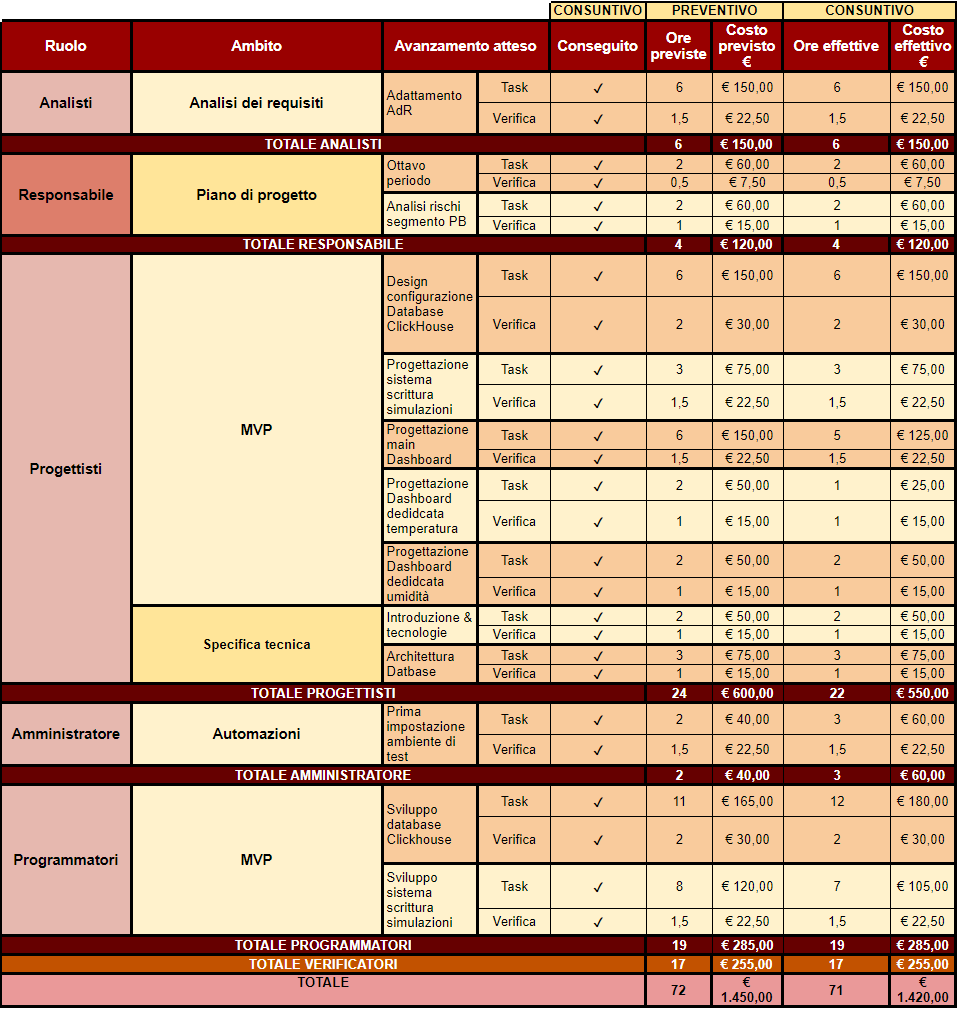
\includegraphics[height=1.1\textwidth]{../Images/periodo8.PNG}
    \caption{Ottavo periodo}
    \label{fig:Ottavo_periodo}
\end{figure}

Al termine dell'ottavo periodo, l'ammontare totale del costo del progetto è \textbf{6012,50\euro} e sono state completate il \textbf{100\%} delle \textit{attività}\textsubscript{\textit{G}} attese.
Il preventivo a finire rimane invariato a \textbf{12425,00\euro} e non risulta necessaria una ripianificazione delle \textit{attività}\textsubscript{\textit{G}} future.
\href{https://github.com/orgs/ByteOps-swe/projects/3/views/1?sortedBy%5Bdirection%5D=asc&sortedBy%5BcolumnId%5D=64182560}{Vai al Diagramma di Gantt.}

\begin{figure}[H]
    \centering
    \begin{minipage}[b]{0.70\textwidth}
        \centering
        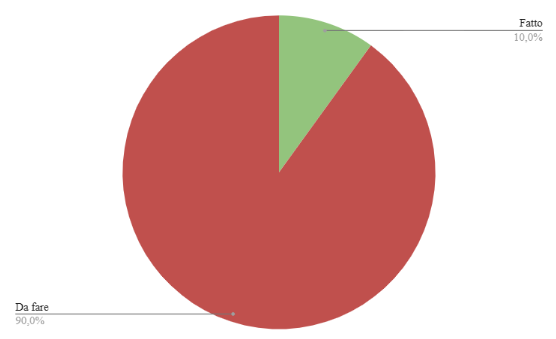
\includegraphics[width=0.7\textwidth]{../Images/avanzamento8Periodo.png}
        \caption{Avanzamento dei lavori RTB - Ottavo periodo}
        \label{fig:Avanzamento_RTB_8}
    \end{minipage}
\end{figure}

\paragraph{Preventivo orario}

\begin{figure}[H] 
    \centering
    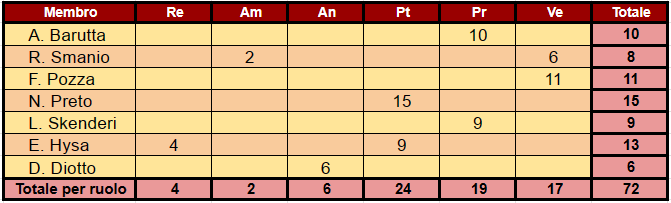
\includegraphics[width=0.9\textwidth]{../Images/preventivoOrario8Periodo.png}
    \caption{Preventivo orario per membro - Ottavo periodo}
    \label{fig:Preventivo_orario_8}
\end{figure}

\begin{figure}[H]
    \centering
    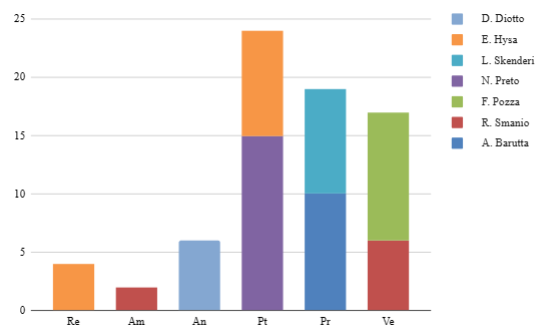
\includegraphics[width=0.6\textwidth]{../Images/preventivoDivisioneRuoli8Periodo.png}
    \caption{Istogramma preventivo della ripartizione oraria dei ruoli - Ottavo periodo}
    \label{fig:Preventivo_ripartizione_oraria_8}
\end{figure}

\paragraph{Consuntivo orario}

\begin{figure}[H]
    \centering
    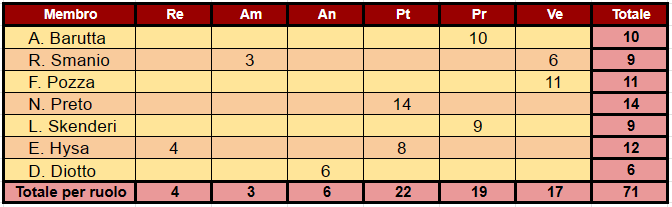
\includegraphics[width=0.9\textwidth]{../Images/consuntivoOrario8Periodo.png}
    \caption{Consuntivo orario per membro - Ottavo periodo}
    \label{fig:Constuntivo_orario_8}
\end{figure}

\begin{figure}[H]
    \centering
    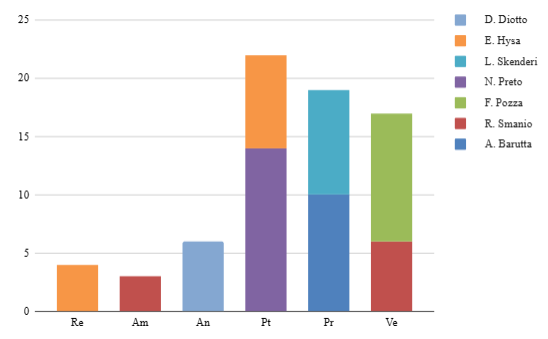
\includegraphics[width=0.6\textwidth]{../Images/consuntivoDivisioneRuoli8Periodo.png}
    \caption{Istogramma consuntivo della ripartizione oraria dei ruoli - Ottavo periodo}
    \label{fig:Consuntivo_ripartizione_oraria_8}
\end{figure}

%---------------------NONO PERIODO---------------------------------------

\subsubsection{Nono periodo  23/02/2024 - 01/03/2024}

\paragraph{Considerazioni}
Durante il nono periodo, sono state dedicate notevoli risorse alle \textit{attività}\textsubscript{\textit{G}} di progettazione, sviluppo e testing relative al Minimum Viable Product (\textit{MVP}\textsubscript{\textit{G}}). \\
I progettisti e gli sviluppatori hanno completato le \textit{attività}\textsubscript{\textit{G}} di progettazione e sviluppo delle \textit{dashboard}\textsubscript{\textit{G}} in \textit{Grafana}\textsubscript{\textit{G}}. Questo ha portato alla realizzazione di una \textit{dashboard}\textsubscript{\textit{G}} principale, concepita per offrire una visione d'insieme dello stato di salute della città, e una \textit{dashboard}\textsubscript{\textit{G}} secondaria, pensata per consentire un'analisi dettagliata delle misurazioni mediante l'applicazione di filtri personalizzati. \\
In seguito al completamento delle \textit{dashboard}\textsubscript{\textit{G}}, è stata avviata la redazione del \textit{Manuale Utente}. È importante notare che le sezioni del \textit{Manuale Utente} redatte nell'attuale periodo non sono state ancora verificate, ma tale verifica è stata pianificata per il periodo successivo, garantendo così una quantità adeguata di materiale da esaminare.
Progettisti e programmatori, oltre alla realizzazione delle \textit{dashboard}\textsubscript{\textit{G}}, hanno portato a termine la progettazione e lo sviluppo del \textit{database}\textsubscript{\textit{G}} e si sono inoltre dedicati all'implementazione della funzionalità di calcolo del punteggio di salute utilizzando la libreria Faust. \\
Per quanto riguarda il documento "\textit{Specifica Tecnica}", sono state completate le sezioni "Introduzione" e "Scelte Tecnologiche" ed è stata avviata la redazione della sezione relativa all'\textit{architettura}\textsubscript{\textit{G}} del \textit{database}\textsubscript{\textit{G}}. \\
Nell'attuale periodo, l'amministratore si è dedicato alla modifica della struttura della \textit{repository}\textsubscript{\textit{G}}, in risposta alle osservazioni ricevute dal Prof. Vardanega durante la revisione \textit{RTB}\textsubscript{\textit{G}}. Grazie a quest'intervento, la \textit{repository}\textsubscript{\textit{G}} è stata resa più semplice e intuitiva, soddisfacendo così le richieste di miglioramento. \\
Parallelamente allo sviluppo delle componenti principali del \textit{sistema}\textsubscript{\textit{G}}, sono stati avviati i \textit{test}\textsubscript{\textit{G}}, con particolare attenzione allo sviluppo dei \textit{test}\textsubscript{\textit{G}} di unità per i simulatori dei sensori e dei \textit{test}\textsubscript{\textit{G}} di \textit{integrazione}\textsubscript{\textit{G}} tra \textit{Python}\textsubscript{\textit{G}} e \textit{Kafka}\textsubscript{\textit{G}} e tra \textit{Python}\textsubscript{\textit{G}} e \textit{Clickhouse}\textsubscript{\textit{G}}.

\paragraph{Gestione dei rischi}

\begin{itemize}
    \item \textbf{Rischi attesi e verificati:}
    \begin{itemize}
        \item \textbf{RO-2A-4} - Inesperienza nell'\textit{attività}\textsubscript{\textit{G}} di testing (\textit{\ref{sec:inexpAttività}})
        \begin{itemize}
            \item \textbf{Esito della mitigazione}: Grazie all'implementazione di sessioni di formazione mirate e all'orientamento fornito dal professore durante il diario di bordo e dall'azienda \textit{proponente}\textsubscript{\textit{G}} durante gli ultimi \textit{SAL}\textsubscript{\textit{G}}, il nostro team ha gradualmente superato le difficoltà iniziali legate all'inesperienza nel testing. \\
            Attraverso la pratica con la realizzazione di minimal working examples sia nel periodo precedente, che in quello attuale, le competenze del team nell'ambito del testing sono notevolmente cresciute. Inoltre, sono state effettuate sessioni di peer-review per favorire lo scambio di conoscenze e migliorare le competenze del team, con particolare attenzione all'\textit{integrazione}\textsubscript{\textit{G}} tra \textit{Python}\textsubscript{\textit{G}} e \textit{Kafka}\textsubscript{\textit{G}}.
            \item \textbf{Impatto}: Nonostante le iniziali difficoltà, l'attuazione delle strategie di mitigazione ha portato a un significativo miglioramento delle competenze del team nella realizzazione dei \textit{test}\textsubscript{\textit{G}}. Questo ha aumentato notevolmente l'efficienza e l'efficacia nell'esecuzione dei \textit{test}\textsubscript{\textit{G}} di \textit{integrazione}\textsubscript{\textit{G}} e ha ridotto il rischio di errori durante lo sviluppo e il rilascio del \textit{software}\textsubscript{\textit{G}}. Inoltre, il processo formativo, seppur dispendioso, ha avuto un impatto positivo sull'intero team, aumentando la consapevolezza e la capacità di affrontare sfide simili in futuro con maggiore sicurezza, velocità e competenza.
        \end{itemize}
    \end{itemize}
\item \textbf{Rischi attesi ma non verificati:}
    \begin{itemize}
        \item \textbf{RO-2A-4} - Inesperienza nell'\textit{attività}\textsubscript{\textit{G}} di progettazione (\textit{\ref{sec:inexpAttività}}) \\
        Il rischio previsto di rallentamenti a causa dell'inesperienza nell'\textit{attività}\textsubscript{\textit{G}} di progettazione non si è verificato. \\
        Le competenze acquisite attraverso la pratica effettuata nel periodo precedente grazie alla realizzazione di minimal working examples hanno agevolato la progettazione del \textit{database}\textsubscript{\textit{G}} e del \textit{sistema}\textsubscript{\textit{G}} di calcolo del punteggio di salute senza il riscontro di particolari difficoltà. Questo risultato evidenzia l'efficacia dell'approccio di formazione e pratica adottato dal team, sottolineando l'importanza dell'investimento continuo nello sviluppo delle competenze del team.
    \end{itemize} 
\item \textbf{Rischi non attesi ma verificati:}
    \begin{itemize}
        \item Nessuno
    \end{itemize}
\end{itemize}


\paragraph{Definizione ruoli}
Per le \textit{attività}\textsubscript{\textit{G}} registrate nei costi, sono stati assegnati i seguenti ruoli: 

\begin{table}[H]
    \centering
    \begin{tabular}{|L{4cm}|L{2cm}|}
        \hline
        \textbf{Ruolo} & \textbf{Persona} \\
        \hline
        \hline
        Responsabile (Re)   & L. Skenderi \\
        \hline
        Amministratore (Am) & F. Pozza \\
        \hline
        Analisti (An)       & L. Skenderi \\
        \hline
        Verificatore (Ve)   & E. Hysa \\
                            & N. Preto \\
                            & A. Barutta \\
                            & L.Skenderi \\   
        \hline
        Programmatori (Pr)  & R. Smanio \\
                            & D. Diotto \\
        \hline
        Progettista (Pt)    & A. Barutta \\
                            & F. Pozza \\
        \hline
    \end{tabular}
    \caption{Tabella dei ruoli assegnati - Nono periodo}
    \label{tab:Ruoli_persone_9}
\end{table}

\paragraph{Pianificazione attività divise per ruoli con consuntivo e preventivo orario e dei costi}

\vspace{0.4cm}

\begin{figure}[H]
    \centering
    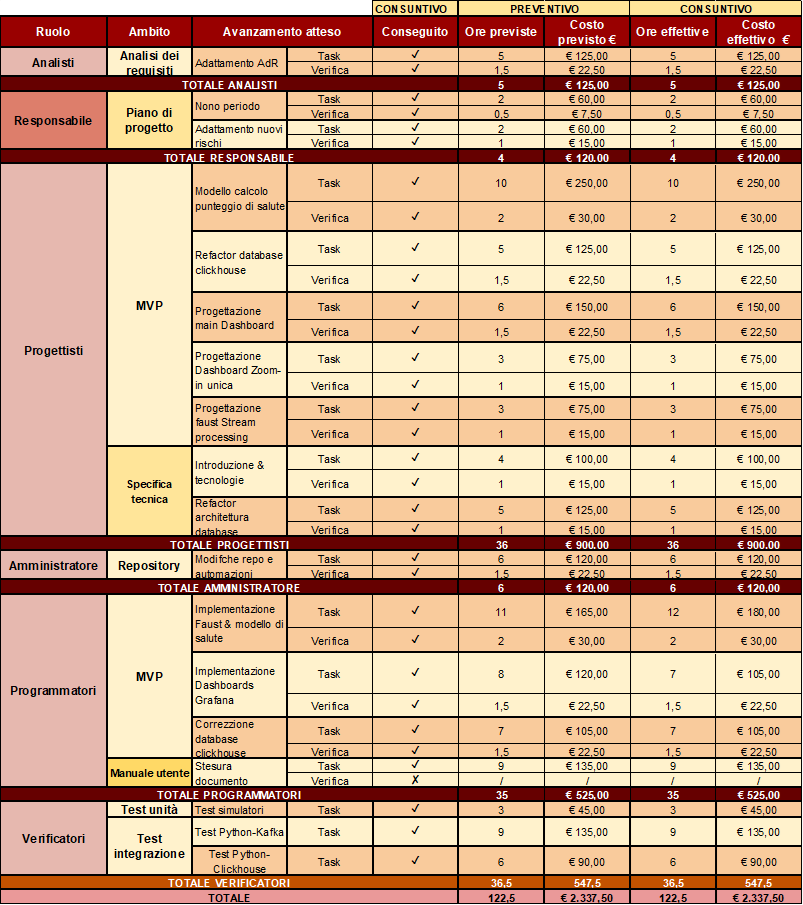
\includegraphics[height=1.1\textwidth]{../Images/periodo9.PNG}
    \caption{Nono periodo}
    \label{fig:Nono_periodo}
\end{figure}

Al termine del nono periodo, l'ammontare totale del costo del progetto è di \textbf{8350 \euro} e sono state completate il \textbf{100\%} delle \textit{attività}\textsubscript{\textit{G}} attese.
Il preventivo a finire rimane invariato a \textbf{12425,00\euro} e non risulta necessaria una ri-pianificazione delle \textit{attività}\textsubscript{\textit{G}} future.
\href{https://github.com/orgs/ByteOps-swe/projects/3/views/1?sortedBy%5Bdirection%5D=asc&sortedBy%5BcolumnId%5D=64182560}{Vai al Diagramma di Gantt.}

\begin{figure}[H]
    \centering
    \begin{minipage}[b]{0.70\textwidth}
        \centering
        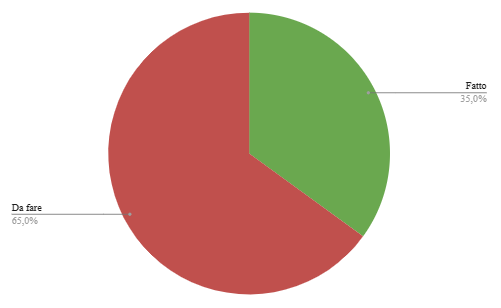
\includegraphics[width=0.7\textwidth]{../Images/avanzamento9Periodo.png}
        \caption{Avanzamento dei lavori RTB - Nono periodo}
        \label{fig:Avanzamento_RTB_9}
    \end{minipage}
\end{figure}

\paragraph{Preventivo orario}

\begin{figure}[H] 
    \centering
    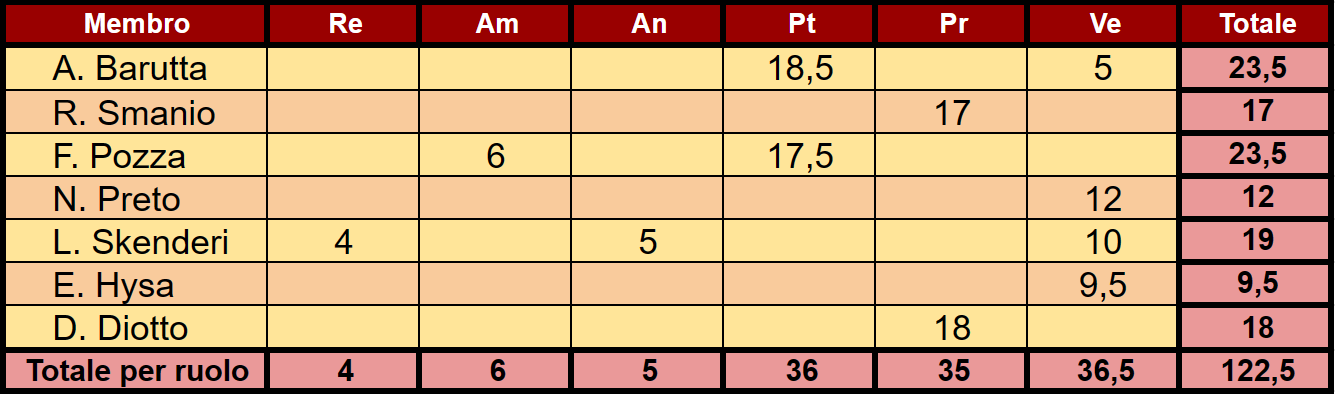
\includegraphics[width=0.9\textwidth]{../Images/preventivoOrario9Periodo.png}
    \caption{Preventivo orario per membro - Nono periodo}
    \label{fig:Preventivo_orario_9}
\end{figure}

\begin{figure}[H]
    \centering
    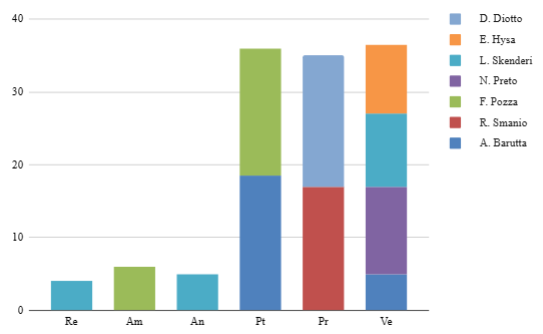
\includegraphics[width=0.6\textwidth]{../Images/preventivoDivisioneRuoli9Periodo.png}
    \caption{Istogramma preventivo della ripartizione oraria dei ruoli - Nono periodo}
    \label{fig:Preventivo_ripartizione_oraria_9}
\end{figure}

\paragraph{Consuntivo orario}

\begin{figure}[H]
    \centering
    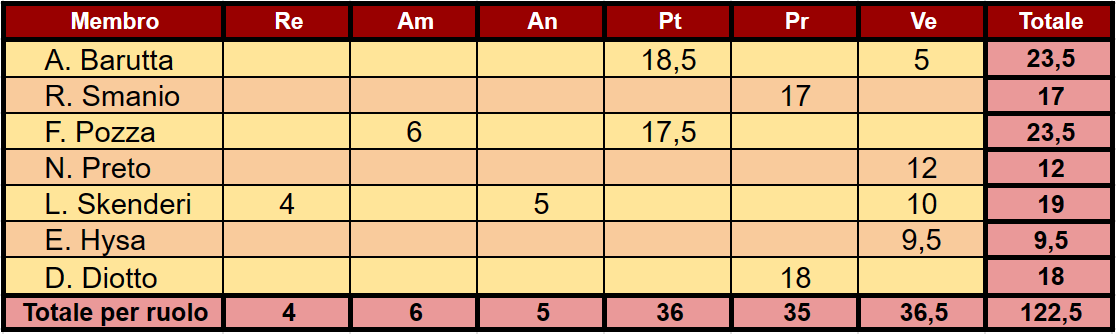
\includegraphics[width=0.9\textwidth]{../Images/consuntivoOrario9Periodo.png}
    \caption{Consuntivo orario per membro - Nono periodo}
    \label{fig:Constuntivo_orario_9}
\end{figure}

\begin{figure}[H]
    \centering
    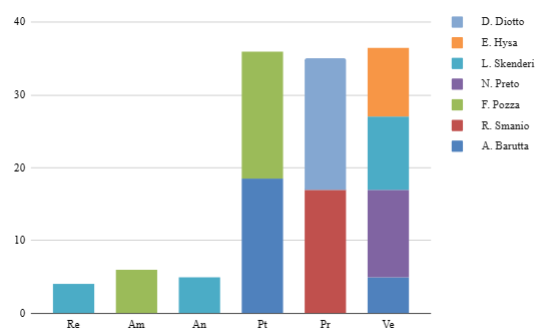
\includegraphics[width=0.6\textwidth]{../Images/consuntivoDivisioneRuoli9Periodo.png}
    \caption{Istogramma consuntivo della ripartizione oraria dei ruoli - Nono periodo}
    \label{fig:Consuntivo_ripartizione_oraria_9}
\end{figure}

%---------------------DECIMO PERIODO---------------------------------------

\subsubsection{Decimo periodo  01/03/2024 - 08/03/2024}

\paragraph{Considerazioni}
Durante il decimo periodo, il team si è dedicato principalmente allo sviluppo dei \textit{test}\textsubscript{\textit{G}} e all'implementazione delle ultime funzionalità in vista della presentazione dell'\textit{MVP}\textsubscript{\textit{G}}. \\
L'Amministratore ha apportato importanti miglioramenti alla pagina GitHub.io, rendendo la presentazione dei documenti e degli artefatti del progetto più intuitiva, seguendo i consigli del Prof. Vardanega emersi durante la revisione \textit{RTB}\textsubscript{\textit{G}}. Inoltre, si è occupato dell'automatizzazione dei \textit{test}\textsubscript{\textit{G}} configurando la pipeline CI per garantire la solidità del processo di \textit{integrazione}\textsubscript{\textit{G}} continua. \\
Il team di progettisti e programmatori ha collaborato per configurare e implementare la funzionalità Time to Live (TTL) nel \textit{database}\textsubscript{\textit{G}} \textit{Clickhouse}\textsubscript{\textit{G}}. Questa funzionalità consente di risparmiare notevolmente spazio di archiviazione, eliminando automaticamente le misurazioni precedenti a un periodo stabilito. Nel nostro caso, questo periodo è di un mese. Tuttavia, anziché eliminare direttamente le misurazioni, prima della loro rimozione definitiva, viene calcolata una media di tali misurazioni per ogni ora. In questo modo, invece di mantenere in memoria tutte le misurazioni meno recenti, viene conservata una sola misurazione aggregata per ogni intervallo orario. Questo approccio assicura un significativo risparmio di spazio di archiviazione nel \textit{database}\textsubscript{\textit{G}}, garantendo al contempo la preservazione di una sintesi delle misurazioni meno recenti, la quale consente l'analisi dei dati anche relativi a periodi molto remoti. \\
I progettisti hanno anche completato la sezione relativa al \textit{database}\textsubscript{\textit{G}} nel documento \textit{Specifica Tecnica} e hanno lavorato attivamente alla progettazione dei \textit{test}\textsubscript{\textit{G}} di unità, di \textit{integrazione}\textsubscript{\textit{G}} e di \textit{sistema}\textsubscript{\textit{G}} per garantire la solidità e l'affidabilità del prodotto. \\
I programmatori hanno implementato filtri per gestire le misurazioni corrotte, migliorando così la stabilità e l'integrità dei dati. Inoltre, hanno aggiunto l'indicazione dell'unità di misura nei grafici sulla \textit{dashboard}\textsubscript{\textit{G}} e apportato miglioramenti grafici per ottimizzare l'esperienza utente. Inoltre, è in corso lo sviluppo di un \textit{sistema}\textsubscript{\textit{G}} per ricevere le notifiche di allerta su \textit{Discord}\textsubscript{\textit{G}} ed è stato completato il \textit{Manuale Utente}. \\
I verificatori hanno svolto un ruolo cruciale nella garanzia della qualità del \textit{software}\textsubscript{\textit{G}}, sviluppando \textit{test}\textsubscript{\textit{G}} sul calcolo del punteggio di salute, \textit{test}\textsubscript{\textit{G}} di \textit{integrazione}\textsubscript{\textit{G}} per verificare l'integrità del flusso dei dati tra \textit{Python}\textsubscript{\textit{G}} e \textit{Kafka}\textsubscript{\textit{G}}, \textit{test}\textsubscript{\textit{G}} sulla gestione dei malfunzionamenti e \textit{test}\textsubscript{\textit{G}} di carico e performance. Si sono anche occupati della verifica del \textit{Manuale Utente} per garantirne chiarezza e usabilità per gli utenti finali. \\
Infine, il Responsabile ha coordinato le \textit{attività}\textsubscript{\textit{G}} del team, assicurandosi che il lavoro svolto fosse in linea con gli obiettivi prefissati. Ha redatto il resoconto del periodo e ha validato il Manuale Utente per assicurare il rispetto degli \textit{standard}\textsubscript{\textit{G}} di qualità richiesti.

\paragraph{Gestione dei rischi}

\begin{itemize}
    \item \textbf{Rischi attesi e verificati:}
        \begin{itemize}
            \item \textbf{RT-1M-4} - Basse prestazioni hardware per i \textit{test}\textsubscript{\textit{G}} di performance (\textit{\ref{sec:lowPrestazioniHW}});
            \begin{itemize}
                \item \textbf{Esito mitigazione}: Data l'assenza di risorse per l'implementazione di un ambiente distribuito e le limitazioni delle macchine disponibili per eseguire \textit{test}\textsubscript{\textit{G}} di carico e performance, non è stato possibile attuare alcuna forma di mitigazione. È stato necessario fare affidamento esclusivamente sulle risorse attualmente disponibili, sebbene sia stato riconosciuto che queste potrebbero non essere sufficienti per condurre \textit{test}\textsubscript{\textit{G}} esaustivi.
                \item \textbf{Impatto}: L'impossibilità di mitigare il rischio ha impattato direttamente sulla capacità del team di valutare accuratamente le prestazioni dell'applicativo attualmente in fase di \textit{test}\textsubscript{\textit{G}}. I \textit{test}\textsubscript{\textit{G}} condotti potrebbero non offrire una rappresentazione completa delle reali condizioni di utilizzo e potrebbero non identificare in modo completo i problemi di prestazioni più critici. È essenziale mantenere consapevolezza di questa limitazione durante il proseguimento del progetto e valutare continuamente alternative per compensare la mancanza di risorse, come l'ottimizzazione del codice o l'adozione di strumenti di simulazione più leggeri.
            \end{itemize}
            \item \textbf{RP-3M-2} - Assenza per ferie del membro dell'azienda \textit{proponente}\textsubscript{\textit{G}} specializzato nelle tecnologie~(\textit{\ref{subsubsec:contattiProponente}})
                \begin{itemize}
                    \item \textbf{Esito mitigazione}: Nonostante l'assenza del membro più esperto dell'azienda \textit{proponente}\textsubscript{\textit{G}} nelle tecnologie utilizzate, il progresso del progetto nel suo complesso non ha subito compromessi significativi. Il team era stato avvisato di questa eventualità in anticipo e si era preparato adeguatamente. Durante i periodi precedenti, erano stati dedicati sforzi considerevoli per risolvere la maggior parte delle questioni e dei dubbi rimanenti.
                    \item \textbf{Impatto}: 
                    Sebbene il membro più esperto dell'azienda \textit{proponente}\textsubscript{\textit{G}}, specializzato nelle tecnologie utilizzate, fosse assente, il lavoro è continuato senza intoppi significativi. Non si sono verificati rallentamenti nel processo decisionale né emergenze di dubbi che richiedessero una risoluzione immediata. Il team ha dimostrato una notevole capacità di adattamento e gestione delle risorse interne per affrontare efficacemente questa situazione.
                \end{itemize}
        \end{itemize}
    \item \textbf{Rischi attesi ma non verificati:} 
        \begin{itemize}
            \item \textbf{RO-2A-4} - Inesperienza nell'\textit{attività}\textsubscript{\textit{G}} di testing (\textit{\ref{sec:inexpAttività}}) \\
            Durante la pianificazione delle \textit{attività}\textsubscript{\textit{G}} di testing, è stato considerato il rischio di rallentamenti dovuti all'inesperienza del team in questo specifico ambito. Tuttavia, questo rischio non si è concretizzato in quanto la formazione e l'esperienza accumulata durante i periodi precedenti si sono rivelate sufficienti per affrontare con successo le sfide legate alle \textit{attività}\textsubscript{\textit{G}} testing pianificate per il periodo attuale.
        \end{itemize}
    \item \textbf{Rischi non attesi ma verificati:}
        \begin{itemize}
            \item Nessuno
        \end{itemize}
\end{itemize}


\paragraph{Definizione ruoli}
Per le \textit{attività}\textsubscript{\textit{G}} registrate nei costi, sono stati assegnati i seguenti ruoli: 

\begin{table}[H]
    \centering
    \begin{tabular}{|L{4cm}|L{2cm}|}
        \hline
        \textbf{Ruolo} & \textbf{Persona} \\
        \hline
        \hline
        Responsabile (Re)   & R. Smanio \\
        \hline
        Amministratore (Am) & E. Hysa \\
        \hline
        Analisti (An)       & N. Preto \\
        \hline
        Verificatore (Ve)   & R. Smanio \\
                            & A. Barutta \\ 
        \hline
        Programmatori (Pr)  & N. Preto \\
                            & E. Hysa \\
                            & F. Pozza \\
        \hline
        Progettista (Pt)    & D. Diotto \\
                            & L. Skenderi \\
        \hline
    \end{tabular}
    \caption{Tabella dei ruoli assegnati - Decimo periodo}
    \label{tab:Ruoli_persone_10}
\end{table}

\paragraph{Pianificazione attività divise per ruoli con consuntivo e preventivo orario e dei costi}

\vspace{0.4cm}

\begin{figure}[H]
    \centering
    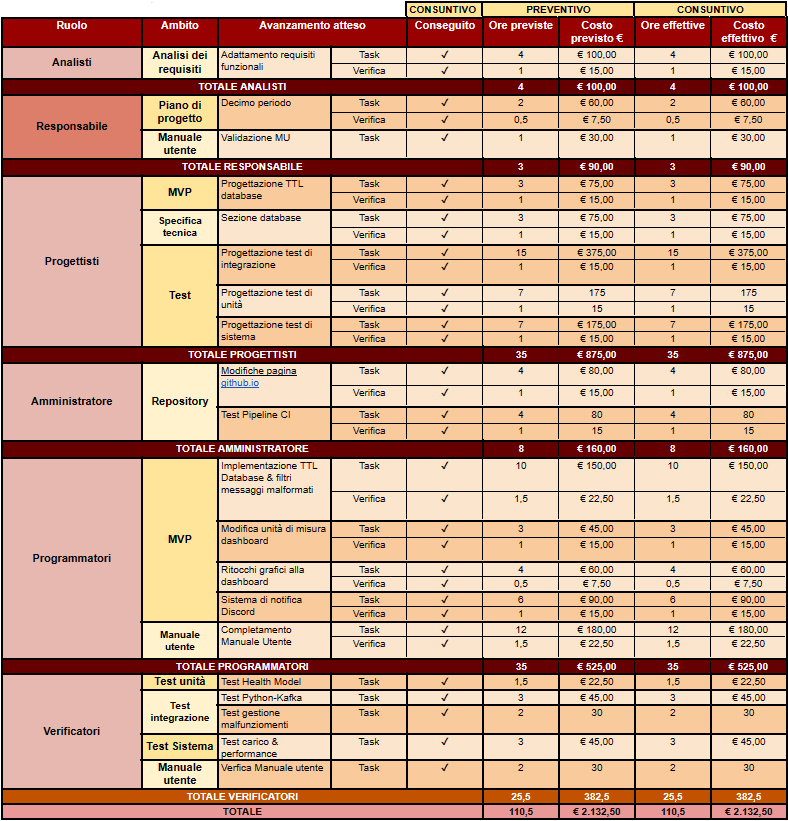
\includegraphics[height=1.1\textwidth]{../Images/periodo10.PNG}
    \caption{Decimo periodo}
    \label{fig:Decimo_periodo}
\end{figure}

Al termine del decimo periodo, l'ammontare totale del costo del progetto è di \textbf{10482.50 \euro} e sono state completate il \textbf{100\%} delle \textit{attività}\textsubscript{\textit{G}} attese.
Il preventivo a finire rimane invariato a \textbf{12425,00\euro} e non risulta necessaria una ri-pianificazione delle \textit{attività}\textsubscript{\textit{G}} future.
\href{https://github.com/orgs/ByteOps-swe/projects/3/views/1?sortedBy%5Bdirection%5D=asc&sortedBy%5BcolumnId%5D=64182560}{Vai al Diagramma di Gantt.}

\begin{figure}[H]
    \centering
    \begin{minipage}[b]{0.70\textwidth}
        \centering
        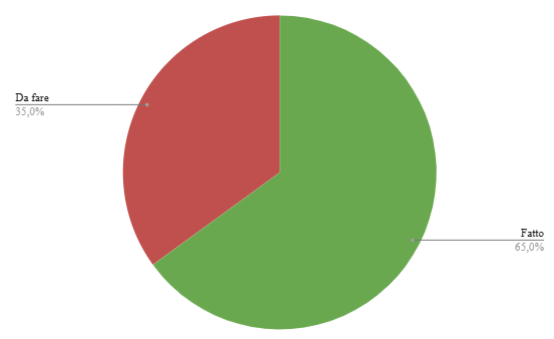
\includegraphics[width=0.7\textwidth]{../Images/avanzamento10Periodo.png}
        \caption{Avanzamento dei lavori RTB - Decimo periodo}
        \label{fig:Avanzamento_RTB_10}
    \end{minipage}
\end{figure}

\paragraph{Preventivo orario}

\begin{figure}[H] 
    \centering
    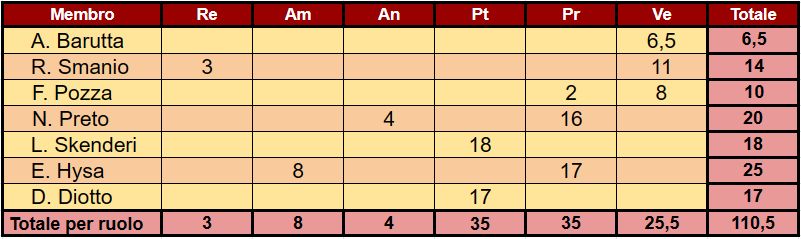
\includegraphics[width=0.9\textwidth]{../Images/preventivoOrario10Periodo.png}
    \caption{Preventivo orario per membro - Decimo periodo}
    \label{fig:Preventivo_orario_10}
\end{figure}

\begin{figure}[H]
    \centering
    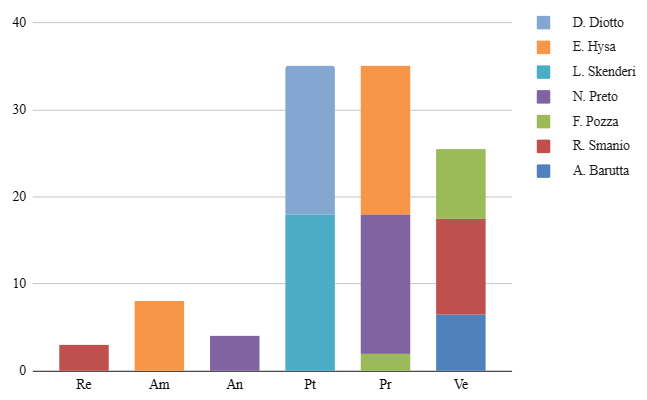
\includegraphics[width=0.6\textwidth]{../Images/preventivoDivisioneRuoli10Periodo.png}
    \caption{Istogramma preventivo della ripartizione oraria dei ruoli - Decimo periodo}
    \label{fig:Preventivo_ripartizione_oraria_10}
\end{figure}

\paragraph{Consuntivo orario}

\begin{figure}[H]
    \centering
    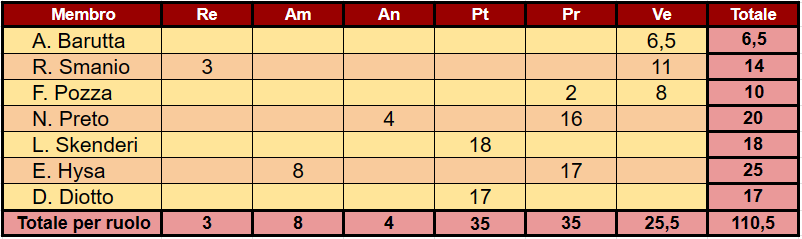
\includegraphics[width=0.9\textwidth]{../Images/consuntivoOrario10Periodo.png}
    \caption{Consuntivo orario per membro - Decimo periodo}
    \label{fig:Constuntivo_orario_10}
\end{figure}

\begin{figure}[H]
    \centering
    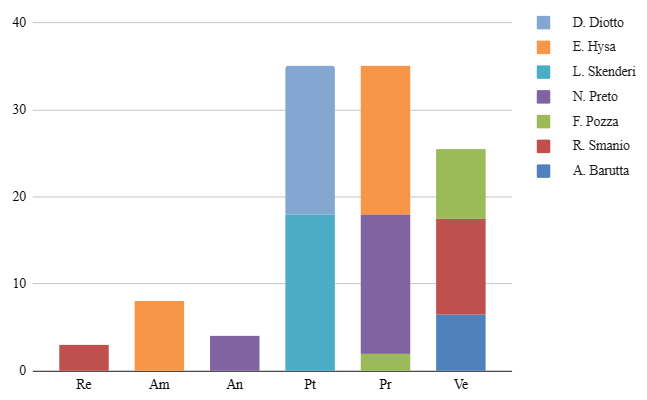
\includegraphics[width=0.6\textwidth]{../Images/consuntivoDivisioneRuoli10Periodo.png}
    \caption{Istogramma consuntivo della ripartizione oraria dei ruoli - Decimo periodo}
    \label{fig:Consuntivo_ripartizione_oraria_10}
\end{figure}

%---------------------UNDICESIMO PERIODO---------------------------------------

\subsubsection{Undicesimo periodo  08/03/2024 - 15/03/2024}

\paragraph{Considerazioni}
Durante l'ultimo periodo, il team ha compiuto importanti progressi e ha raggiunto obiettivi significativi nell'avanzamento del progetto.
Gli analisti hanno completato il documento "\textit{Analisi dei Requisiti v.2.0.0}", fornendo una base solida per la comprensione dei requisiti del progetto. \\
Il Responsabile si è occupato della redazione dell'undicesimo periodo del Piano di Progetto e del coordinamento del team durante questo periodo. \\
I progettisti,  dopo aver definito dettagliatamente l'\textit{architettura}\textsubscript{\textit{G}} di implementazione e di deployment, si sono occupati della redazione delle rispettive sezioni nel documento “\textit{Specifica Tecnica}”. In aggiunta, hanno curato la stesura della sezione "Requisiti soddisfatti" e hanno realizzato dettagliati diagrammi \textit{UML}\textsubscript{\textit{G}} per tutte le classi. Questo lavoro ha fornito una guida chiara e dettagliata per la comprensione dell'\textit{architettura}\textsubscript{\textit{G}} del \textit{sistema}\textsubscript{\textit{G}}, fondamentale per un avanzamento coerente e ben orientato dello sviluppo del progetto. \\
L'amministratore ha introdotto miglioramenti significative nella \textit{repository}\textsubscript{\textit{G}}, tra cui il completamento della pagina \textit{github}\textsubscript{\textit{G}}.io e l'inserimento di badge GitHub e della pipeline CI nel file README.md. 
Queste azioni hanno notevolmente migliorato l'esposizione della \textit{repository}\textsubscript{\textit{G}}, rendendo la presentazione dei documenti e degli artefatti più accessibile e intuitiva per tutti i membri del team e per gli utenti esterni. L'inserimento dei badge relativi ai \textit{test}\textsubscript{\textit{G}} ha fornito una trasparenza aggiuntiva sullo stato del progetto, permettendo a tutti di valutare rapidamente l'affidabilità del codice e l'esito dei \textit{test}\textsubscript{\textit{G}} effettuati. Tale trasparenza non solo favorisce una migliore comprensione del lavoro svolto, ma anche una maggiore fiducia nella qualità complessiva del \textit{software}\textsubscript{\textit{G}} in sviluppo. \\
I programmatori si sono occupati dell’ottimizzazione del codice seguendo le migliori pratiche di sviluppo del \textit{software}\textsubscript{\textit{G}}, garantendo la sua robustezza e sicurezza per semplificare l'\textit{attività}\textsubscript{\textit{G}} di analisi statica da parte dei verificatori. Inoltre, è stato reso thread-safe per gestire efficacemente i \textit{processi}\textsubscript{\textit{G}} concorrenti. Sono stati apportati miglioramenti grafici per migliorare l'esperienza utente sulla \textit{dashboard}\textsubscript{\textit{G}} e il \textit{sistema}\textsubscript{\textit{G}} di notifica tramite \textit{Discord}\textsubscript{\textit{G}} è stato implementato con successo. \\
I verificatori hanno svolto un ruolo cruciale nel garantire la qualità del \textit{software}\textsubscript{\textit{G}}, completando tutti i \textit{test}\textsubscript{\textit{G}} necessari, inclusi quelli di unità, \textit{integrazione}\textsubscript{\textit{G}}, \textit{sistema}\textsubscript{\textit{G}}, carico e performance. \\
In conclusione, il team ha dimostrato un impegno costante, una collaborazione efficace e un'attenzione scrupolosa ai dettagli durante questo periodo. Questi fattori hanno contribuito in modo significativo a stabilire una base solida per il proseguimento del progetto verso la sua conclusione. L'accento posto sulla qualità del risultato finale è stato un punto focale in ogni fase del lavoro, garantendo che il prodotto finale risponda in modo adeguato alle aspettative e ai requisiti del cliente.


\paragraph{Gestione dei rischi}

\begin{itemize}
    \item \textbf{Rischi attesi e verificati:}
        \begin{itemize}
            \item \textbf{RP-2B-1} - Divergenze nella redazione del documento \textit{Specifica Tecnica}~(\textit{\ref{subsubsec:contrastiInterni}}).
            \begin{itemize}
                \item \textbf{Esito mitigazione}: durante la redazione del documento \textit{Specifica Tecnica}, il team ha riscontrato divergenze riguardanti la struttura e i contenuti di alcune sezioni. Per affrontare questa situazione, il Responsabile ha organizzato una votazione per concordare su una struttura comune e risolvere le divergenze.
                \item \textbf{Impatto}: grazie alla votazione guidata dal Responsabile, le divergenze sono state risolte in modo efficace, garantendo coerenza e coesione nel documento. Ciò ha permesso al team di proseguire senza ritardi nella redazione e ha assicurato la qualità complessiva della \textit{Specifica Tecnica}.
            \end{itemize}
            
        \end{itemize}
    \item \textbf{Rischi attesi ma non verificati:}
        \begin{itemize}
            \item \textbf{RP-3M-2} - Assenza per ferie del membro dell'azienda \textit{proponente}\textsubscript{\textit{G}} specializzato nelle tecnologie~(\textit{\ref{subsubsec:contattiProponente}})
                \begin{itemize}
                    \item \textbf{Esito mitigazione}: come evidenziato nella precedente fase, l'impatto di questo rischio è stato attenuato grazie alle adeguate precauzioni adottate. In particolare, non si sono manifestati dubbi o domande riguardanti potenziali problemi con le tecnologie utilizzate.
                    \item \textbf{Impatto}: 
                    le misure preventive adottate hanno limitato l'impatto del rischio sul progetto.
                \end{itemize}
        \end{itemize}
    \item \textbf{Rischi non attesi ma verificati:}
        \begin{itemize}
            \item Nessuno
        \end{itemize}
\end{itemize}


\paragraph{Definizione ruoli}
Per le \textit{attività}\textsubscript{\textit{G}} registrate nei costi, sono stati assegnati i seguenti ruoli: 

\begin{table}[H]
    \centering
    \begin{tabular}{|L{4cm}|L{2cm}|}
        \hline
        \textbf{Ruolo} & \textbf{Persona} \\
        \hline
        \hline
        Responsabile (Re)   & D. Diotto \\
        \hline
        Amministratore (Am) & N. Preto \\
        \hline
        Analisti (An)       & E. Hysa \\
        \hline
        Verificatore (Ve)   & D. Diotto \\
                            & A. Barutta \\ 
        \hline
        Programmatori (Pr)  & L. Skenderi \\
                            & F. Pozza \\
        \hline
        Progettista (Pt)    & R. Smanio \\
                            & E. Hysa \\
        \hline
    \end{tabular}
    \caption{Tabella dei ruoli assegnati - Undicesimo periodo}
    \label{tab:Ruoli_persone_11}
\end{table}

\paragraph{Pianificazione attività divise per ruoli con consuntivo e preventivo orario e dei costi}

\vspace{0.4cm}

\begin{figure}[H]
    \centering
    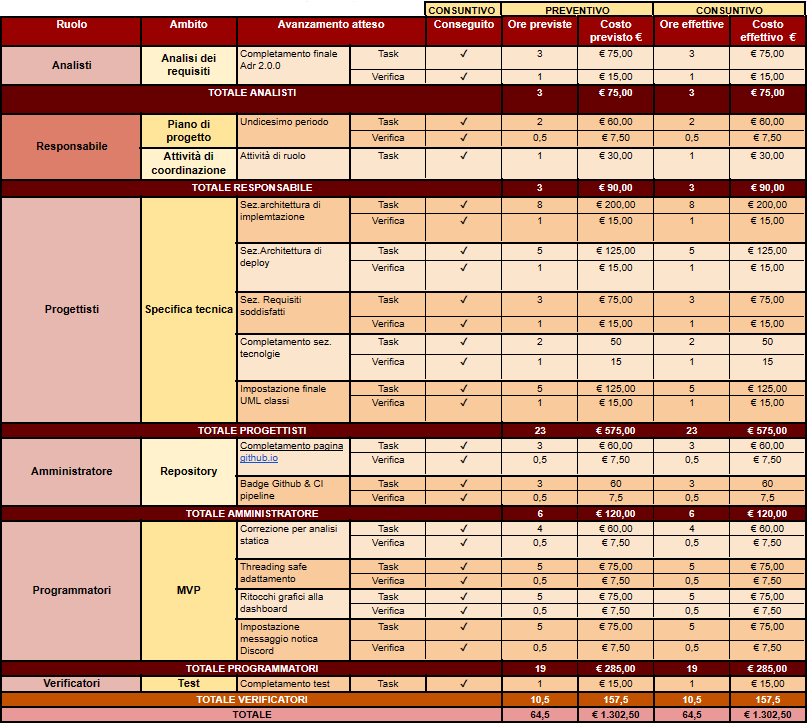
\includegraphics[height=0.9\textwidth]{../Images/periodo11.PNG}
    \caption{Undicesimo periodo}
    \label{fig:Undicesimo_periodo}
\end{figure}

Al termine del decimo periodo, l'ammontare totale del costo del progetto è di \textbf{11785 \euro} e sono state completate il \textbf{100\%} delle \textit{attività}\textsubscript{\textit{G}} attese.
Il preventivo a finire rimane invariato a \textbf{12425,00\euro} e non risulta necessaria una ri-pianificazione delle \textit{attività}\textsubscript{\textit{G}} future.
\href{https://github.com/orgs/ByteOps-swe/projects/3/views/1?sortedBy%5Bdirection%5D=asc&sortedBy%5BcolumnId%5D=64182560}{Vai al Diagramma di Gantt.}

\begin{figure}[H]
    \centering
    \begin{minipage}[b]{0.70\textwidth}
        \centering
        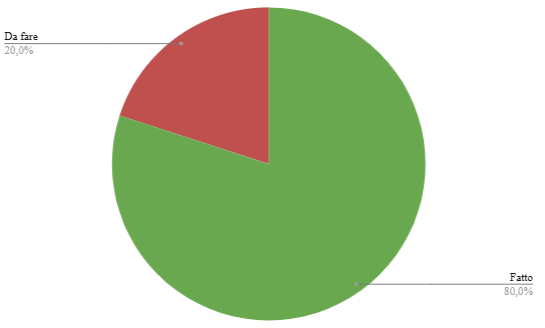
\includegraphics[width=0.7\textwidth]{../Images/avanzamento11Periodo.png}
        \caption{Avanzamento dei lavori RTB - Undicesimo periodo}
        \label{fig:Avanzamento_RTB_11}
    \end{minipage}
\end{figure}

\paragraph{Preventivo orario}

\begin{figure}[H] 
    \centering
    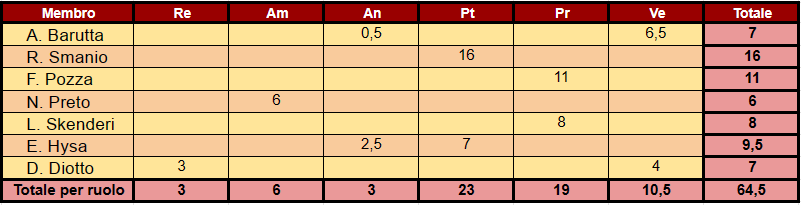
\includegraphics[width=0.9\textwidth]{../Images/preventivoOrario11Periodo.png}
    \caption{Preventivo orario per membro - Undicesimo periodo}
    \label{fig:Preventivo_orario_11}
\end{figure}

\begin{figure}[H]
    \centering
    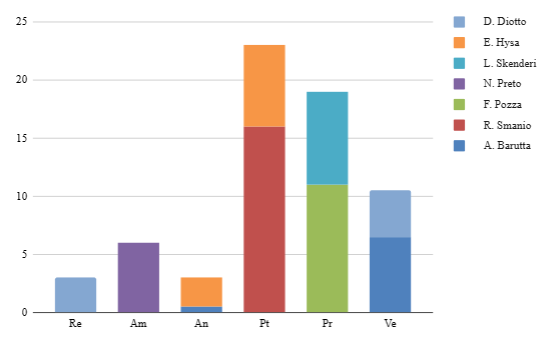
\includegraphics[width=0.6\textwidth]{../Images/preventivoDivisioneRuoli11Periodo.png}
    \caption{Istogramma preventivo della ripartizione oraria dei ruoli - Undicesimo periodo}
    \label{fig:Preventivo_ripartizione_oraria_11}
\end{figure}

\paragraph{Consuntivo orario}

\begin{figure}[H]
    \centering
    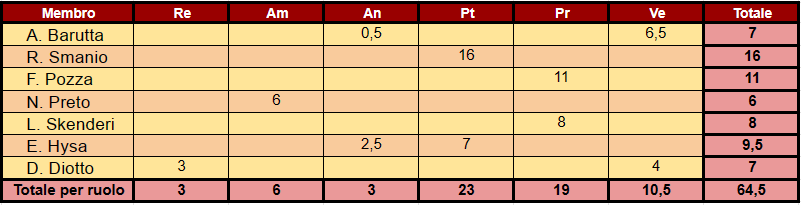
\includegraphics[width=0.9\textwidth]{../Images/consuntivoOrario11Periodo.png}
    \caption{Consuntivo orario per membro - Undicesimo periodo}
    \label{fig:Constuntivo_orario_11}
\end{figure}

\begin{figure}[H]
    \centering
    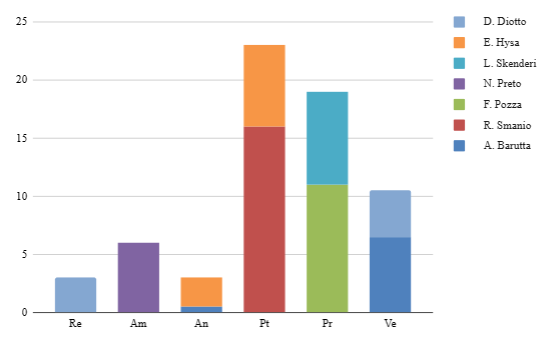
\includegraphics[width=0.6\textwidth]{../Images/consuntivoDivisioneRuoli11Periodo.png}
    \caption{Istogramma consuntivo della ripartizione oraria dei ruoli - Undicesimo periodo}
    \label{fig:Consuntivo_ripartizione_oraria_11}
\end{figure}

%---------------------DODICESIMO PERIODO---------------------------------------

\subsubsection{Dodicesimo periodo  15/03/2024 - 22/03/2024}

\paragraph{Considerazioni}
Relativamente al dodicesimo periodo, i principali obiettivi programmati consistono nell'avanzamento della redazione di \textit{Specifica Tecnica}, che si avvicina alla fase conclusiva, e nell'allocazione di risorse significative per migliorare la robustezza e l'affidabilità del sistema.

Il responsabile ha svolto un ruolo cruciale nel coordinare il team e nella redazione dettagliata dell'attuale periodo all'interno del documento "\textit{Piano di Progetto}".

I progettisti si sono occupati della redazione del documento \textit{Specifica Tecnica}. Nello specifico sono state redatte le sezioni "Schema Registry", "Database Configuration", "Faust", "Architettura Simulatori", "Kafka" e "Grafana". Questo sottolinea il loro ruolo centrale nella definizione dell'architettura e delle specifiche tecniche, fondamentali per la comprensione e per lo sviluppo del prodotto.

L'amministratore ha configurato l'ambiente containerizzato per garantire l'operatività ottimale e l'integrazione corretta dello Schema Registry e di Zookeeper, contribuendo così a garantire la robustezza e la resilienza del sistema.

I programmatori si sono dedicati all'implementazione dello Schema Registry e all'integrazione di quest’ultimo con lo script Python utilizzato per scrivere nei topic Kafka, al fine di validare il formato dei messaggi direttamente alla fonte. Questo approccio assicura che i messaggi siano validati prima di essere inviati al topic Kafka, evitando così un sovraccarico di rete inutile.

Lo Schema Registry svolge un ruolo cruciale nel mantenere la coerenza e l'integrità dei dati, consentendo una gestione centralizzata degli schemi utilizzati all'interno dell'ecosistema dei dati. Questa implementazione e la relativa validazione sono fondamentali per garantire che i messaggi trasmessi siano conformi agli standard definiti, prevenendo l'inserimento di dati errati o incompatibili nel sistema, e aumentando l'affidabilità complessiva del sistema.

In conclusione, è importante sottolineare che ogni richiesta formulata dall’azienda proponente è stata diligentemente affrontata e risolta nei tempi concordati, determinando così il raggiungimento del completamento dell'MVP. Tale risultato non solo evidenzia l’impegno del team nel soddisfare le aspettative del cliente, ma anche la capacità di rispondere in modo tempestivo e efficace alle esigenze del progetto.


\paragraph{Gestione dei rischi}

\begin{itemize}
    \item \textbf{Rischi attesi e verificati:}
        \begin{itemize}
            \item Nessuno.
        \end{itemize}
    \item \textbf{Rischi attesi ma non verificati:}
        \begin{itemize}
            \item \textbf{RP-2B-1} - Contrasti interni al gruppo~(\S\textit{\ref{subsubsec:contrastiInterni}}) \\
            Era prevista la possibilità di contrasti interni al gruppo dovuti al notevole numero di sezioni da redigere. In particolare, si temeva che potessero sorgere divergenze riguardo la struttura delle varie sezioni e la modalità di presentazione delle informazioni. Tuttavia, questa eventualità non si è concretizzata poiché il team è stato in grado di collaborare in modo efficace e coeso, mantenendo un'armonia nell'approccio alla redazione delle sezioni, il che ha contribuito positivamente al progresso complessivo della redazione del documento.
            \item \textbf{RT-1A-1} - Difficoltà nell’implementazione dello Schema Registry~(\S\textit{\ref{sec:rischioTec}}) \\
            L'implementazione dello Schema Registry si presentava inizialmente complessa, essendo una funzionalità introdotta in extremis per rafforzare la robustezza del sistema. Inoltre, la ristrettezza dei tempi a disposizione alimentava ragionevolmente dubbi sulla sua fattibilità. Tuttavia, non si sono verificati ostacoli significativi, e si è proceduto senza intoppi, raggiungendo gli obiettivi prefissati con successo.
        \end{itemize}
    \item \textbf{Rischi non attesi ma verificati:}
        \begin{itemize}
            \item \textbf{RO-1A-1} - Assenza di un componente del team per 3 giorni~(\S\textit{\ref{sec:ImpPersonali}})
                \begin{itemize}
                    \item \textbf{Esito mitigazione}: L'assenza di uno dei membri del team non si è rivelata problematica in quanto il resto del team è stato in grado di gestire efficacemente le responsabilità del membro assente durante il periodo di assenza. Grazie all'intervento tempestivo del responsabile, che ha riassegnato i compiti del membro assente in modo efficace, il team è riuscito a raggiungere gli obiettivi prefissati senza rallentamenti.
                    \item \textbf{Impatto}: L'assenza temporanea del membro del team non ha avuto un impatto significativo sullo sviluppo del progetto, poiché le attività sono proseguite senza interruzioni e gli obiettivi sono stati raggiunti nei tempi previsti.
                \end{itemize}
        \end{itemize}
\end{itemize}

\paragraph{Definizione ruoli}
Per le \textit{attività}\textsubscript{\textit{G}} registrate nei costi, sono stati assegnati i seguenti ruoli: 

\begin{table}[H]
    \centering
    \begin{tabular}{|L{4cm}|L{2cm}|}
        \hline
        \textbf{Ruolo} & \textbf{Persona} \\
        \hline
        \hline
        Responsabile (Re)   & A. Barutta \\
        \hline
        Amministratore (Am) & R. Smanio \\
        \hline
        Verificatore (Ve)   & D. Diotto \\
                            & E. Hysa \\
                            & A. Barutta \\
                            & L. Skenderi \\ 
        \hline
        Programmatore (Pr)  & A. Barutta \\
                            & F. Pozza \\
        \hline
        Progettista (Pt)    & N. Preto \\
                            & E. Hysa \\
        \hline
    \end{tabular}
    \caption{Tabella dei ruoli assegnati - Dodicesimo periodo}
    \label{tab:Ruoli_persone_12}
\end{table}

\paragraph{Pianificazione attività divise per ruoli con consuntivo e preventivo orario e dei costi}

\vspace{0.4cm}

\begin{figure}[H]
    \centering
    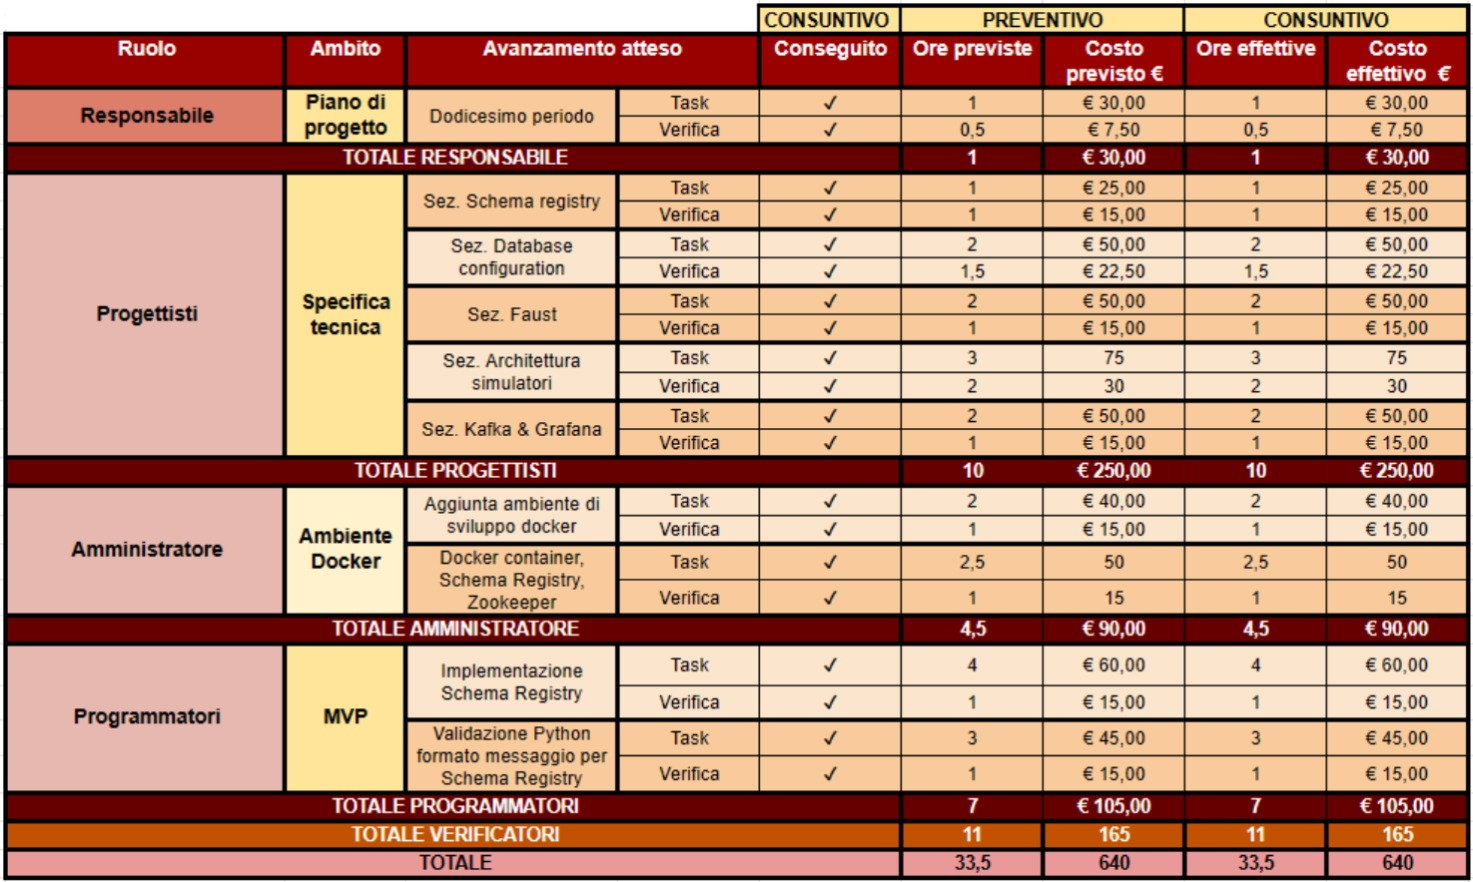
\includegraphics[height=0.6\textwidth]{../Images/periodo12.jpeg}
    \caption{Dodicesimo periodo}
    \label{fig:Dodicesimo_periodo}
\end{figure}

Al termine del decimo periodo, l'ammontare totale del costo del progetto è di \textbf{12425 \euro} e sono state completate il \textbf{100\%} delle \textit{attività}\textsubscript{\textit{G}} attese.
Il preventivo a finire rimane invariato a \textbf{12425,00\euro} e non risulta necessaria una ri-pianificazione delle \textit{attività}\textsubscript{\textit{G}} future.
\href{https://github.com/orgs/ByteOps-swe/projects/3/views/1?sortedBy%5Bdirection%5D=asc&sortedBy%5BcolumnId%5D=64182560}{Vai al Diagramma di Gantt.}

\begin{figure}[H]
    \centering
    \begin{minipage}[b]{0.70\textwidth}
        \centering
        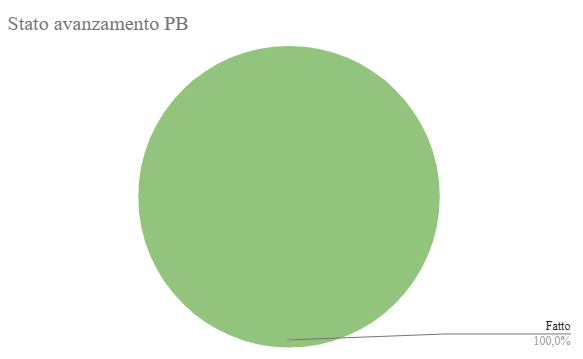
\includegraphics[width=0.9\textwidth]{../Images/avanzamento12Periodo.png}
        \caption{Avanzamento dei lavori RTB - Dodicesimo periodo}
        \label{fig:Avanzamento_RTB_12}
    \end{minipage}
\end{figure}

\paragraph{Preventivo orario}

\begin{figure}[H] 
    \centering
    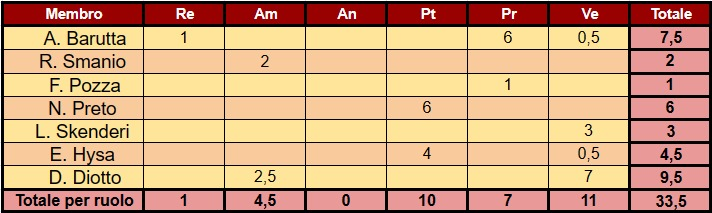
\includegraphics[width=0.9\textwidth]{../Images/preventivoOrario12Periodo.jpeg}
    \caption{Preventivo orario per membro - Dodicesimo periodo}
    \label{fig:Preventivo_orario_12}
\end{figure}

\begin{figure}[H]
    \centering
    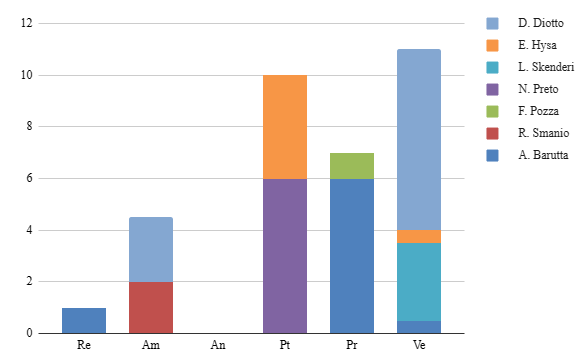
\includegraphics[width=0.8\textwidth]{../Images/preventivoDivisioneRuoli12Periodo.png}
    \caption{Istogramma preventivo della ripartizione oraria dei ruoli - Dodicesimo periodo}
    \label{fig:Preventivo_ripartizione_oraria_12}
\end{figure}

\paragraph{Consuntivo orario}

\begin{figure}[H]
    \centering
    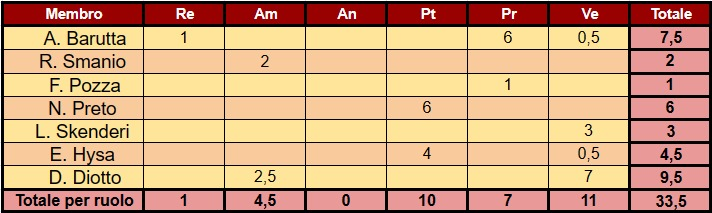
\includegraphics[width=0.9\textwidth]{../Images/consuntivoOrario12Periodo.jpeg}
    \caption{Consuntivo orario per membro - Dodicesimo periodo}
    \label{fig:Constuntivo_orario_12}
\end{figure}

\begin{figure}[H]
    \centering
    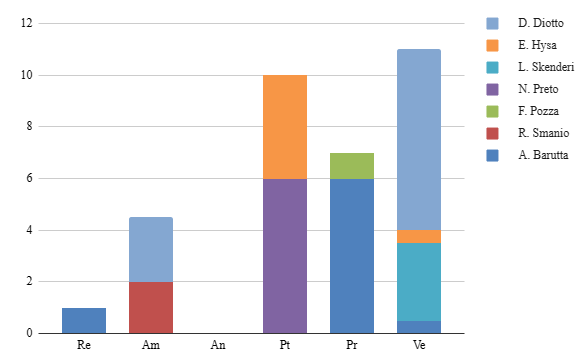
\includegraphics[width=0.8\textwidth]{../Images/consuntivoDivisioneRuoli12Periodo.png}
    \caption{Istogramma consuntivo della ripartizione oraria dei ruoli - Dodicesimo periodo}
    \label{fig:Consuntivo_ripartizione_oraria_12}
\end{figure}